\section{Architektura, TODO: doplnit další zdroje}
Jedno z prvních rozhodnutí, které bylo v souvislosti s návrhem aplikace potřeba udělat, se týkalo architektury aplikace. Dle \cite{twa_architecture} se v případě webových aplikací můžeme setkat s rozdělením na thin-client (smart-server) a thick-client (dump-server). První zmíněná možnost znamená, že veškerá logika se nachází na straně serveru. Pokud se aplikace na straně serveru neskládá z více samostatně fungujících částí, můžeme se také setkat s označením monolitická aplikace. U možnosti thick-client (dump-server) je naopak aplikace na straně klienta a server poskytuje pouze API pro účely komunikace.

Monolitické aplikace nejsou v dnešní době již tak populární, jako tomu bylo v minulosti, nicméně stále mají své uplatnění. Typicky se monolitická architektura využívá u malých aplikací, u kterých se v budoucnu nepředpokládá větší rozšiřování. Jednou z výhod je jistě fakt, že monolitické aplikace se rychleji vyvíjejí a také se jednodušeji testují. Jejich nevýhodou může být naopak složitější údržba a problémové škálování. \cite{twa_architecture} Jelikož je vyvíjená aplikace zamýšlená pouze pro jednotlivé sportovní kluby a nepředpokládá se potřeba přistupovat a upravovat data jiným způsobem než z webového rozhraní nové aplikace, tak jsem se i s ohledem na rychlejší vývoj rozhodl využít monolitickou architekturu.

Výběr této architektury však neznamená, že by nemohla být aplikace vnitřně žádným způsobem členěna. Nějaká forma rozdělení je naopak i žádoucí, aby se oddělila odpovědnost a vznikla určitá forma abstrakce nad jednotlivými částmi systému. Díky tomu je například možné vyměnit datové úložiště bez dalších změn v částech, které se zabývají uživatelským rozhraním nebo obsahují samotnou logiku aplikace. Jednou z možností takového strukturování je využití architektury MVC.

\subsection{MVC architektura}
Následující část textu vychází ze zdrojů \cite{it_network_mvc, mdn_mvc}. Architektura MVC (zkratka pro model-view-controller) odděluje datový model aplikace od řídící logiky a prezentační vrstvy s uživatelským rozhraním. Nejvíce se uchytila u webových aplikací, poněvadž je součástí i mnoha webových frameworků. Na MVC architektuře jsou například založeny frameworky Laravel a Symfony (PHP), ASP.NET MVC framework a mnoho dalších.

MVC architektura se tedy skládá ze tří komponent. Vrstva modelů definuje s jakými daty bude aplikace pracovat. Může také obsahovat validační pravidla pro tato data, případně i další funkce, které se váží k danému modelu (příkladem by mohla být funkce na výpočet věku z informace o datu narození). Při využití objektově relačního mapování kopírují modely z velké části strukturu tabulek v databázi. Jeden model typicky představuje konkrétní tabulku a jednotlivé atributy modelu představují sloupce dané tabulky.

Pohledy (views) se starají o zobrazení dat uživateli. V případě webových aplikací bývá součástí pohledu šablona obsahující HTML, do které jsou následně vkládána data z modelů.

Controllery obsahují logiku, jež se stará o načítání dat z modelů a jejich aktualizaci v závislosti na vstupu od uživatele. Propojují všechny ostatní vrstvy do funkčního celku.

\begin{figure}[h]
	\caption{Životní cyklus požadavku}
	\label{figure:mvc}
	\centering
	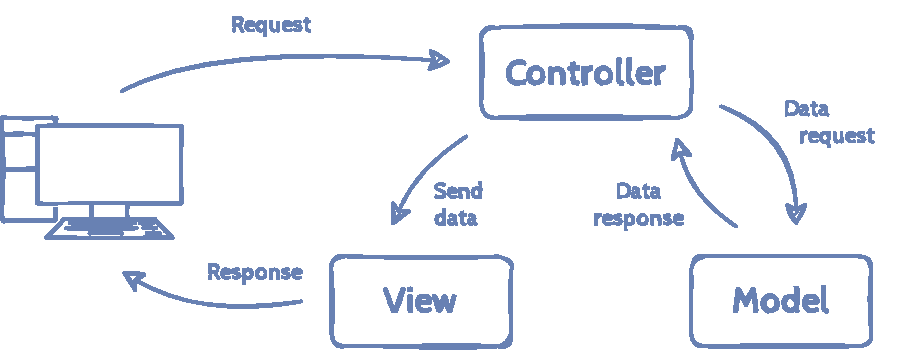
\includegraphics[width=0.9\textwidth]{images/mvc.pdf}
\end{figure}

Obrázek \ref{figure:mvc} zobrazuje typický životní cyklus požadavku. Můžeme si například představit situaci, kdy si uživatel chce zobrazit nadcházející události evidované v aplikaci. Požadavek od uživatele nejdříve zachytí router, který na základě URL adresy rozpozná, jakému controlleru požadavek předat. Daný controller si následně od konkrétního modelu vyžádá uložená data o nadcházejících událostech. Poté, co je od modelu získá, předá tato data pohledu, který je již pouze vloží do připravené šablony. Sestavená stránka je nakonec zaslána zpět uživateli.
